\documentclass[letterpaper,11pt]{article}
\setlength{\textwidth}{6.5in}
\setlength{\hoffset}{0in}
%TODO: tweak these a bit more
\setlength{\voffset}{-0.5in}
\setlength{\textheight}{8.75in}
\setlength{\marginparsep}{0in}
\setlength{\marginparwidth}{0in}
\setlength{\oddsidemargin}{0in}

\usepackage{aas_macros}
\usepackage{amssymb}
\usepackage{caption}
\usepackage{hyperref}
\usepackage{listings}
\usepackage{mathabx}
\usepackage{setspace}
\doublespacing
\usepackage{siunitx}
\DeclareSIUnit\solarradius{R_\Sun}
\DeclareSIUnit\solarmass{M_\Sun}
\usepackage{subcaption}
\usepackage{tabularx}


\usepackage{graphicx}
\usepackage{lineno}
\usepackage[authoryear,square,colon]{natbib}
\bibpunct{[}{]}{;}{a}{,}{,~}

\usepackage{lipsum}

\begin{document}


\title{Searching for the $E^{-3/2}$ Suprathermal Power Law Tail in Parker Solar Probe's IS$\Sun$IS Data}
\author{A. Merrill}
\date{\today}
\maketitle

\linenumbers

\begin{abstract}
The  \textit{Advanced  Composition  Explorer} (ACE)  and  the  \textit{Ulysses}  spacecraft revealed the presence of a common power-law spectrum of ions in the solar wind, the shape of which is independent of solar activity.  The highest energy particles in this distribution are a direct interest to human affairs as they can serve as the seed population for large, destructive events that can harm ground- and air-based equipment.  The mechanisms that create this common distribution are unknown, but by studying the behavior of the spectrum  at  closer  radii  more  can  be  learned  about  their  origin.  Furthermore, this relationship is altogether poorly studied within \SI{1}{\astronomicalunit}.  I investigate the first year and a half of Parker Solar Probe's data to find evidence of this spectrum in this previously unstudied region. I find weak evidence to suggest the existence of a common spectrum of protons from 60 to \SI{200}{\kilo\electronvolt} inside the region being studied.  Further work is required to uncover the phenomena  in  this  region  that  determine  the  shape  of  the  solar  wind spectra.
\end{abstract}



\section{Introduction}
\label{sec:intro}
The solar wind in regions above \SI{0.3}{\astronomicalunit} has been studied directly~\citep{McComas2007}, and a considerable understanding of the population of solar wind particles and their distributions has been gained about these regions~\citep{Giacalone2002,Fisk2012,Fisk2006,Fisk2008,Gloeckler2000}.  One particular phenomenon that our current understanding of accelerating processes in the solar wind fails to explain is the existence of an omnipresent power law spectrum of solar wind speed with a spectral index of $-5$; alternatively, this can be expressed as a power law of particle energy with spectral index of $-{3 \over 2}$~\citep{Fisk2012}.

\subsection{Acceleration of Solar Energetic Particles}
There are at least two mechanisms that accelerate solar energetic particles (SEPs) that are capable of working over a broad spectrum of energies (a few \si{\kilo\electronvolt} to \si{\giga\electronvolt}).  Implusive SEPs can result from magnetic-reconnection driven processes occurring during solar flares.  Gradual SEP events can be created from coronal mass ejection-driven shocks~\citep{Desai2016}.  However, the mechanics of either of these types of acceleration cannot produce the seemingly omnipresent power-law with index $-{3 \over 2}$.

A seed population of suprathermal particles (ie. \SI{>10}{\kilo\electronvolt}) is responsible for the acceleration of most solar energetic particles (SEPs), rather than the bulk solar wind~\citep{Mewaldt2012}.  The seed population for SEP events is of particular interest to human affairs as large SEP events can cause significant harm to humans and machinery in space and, in extreme circumstances, even those on the ground~\citep{Desai2016}.  This seed population is directly concerned with the power law spectrum seen in the solar wind as the seed population for SEP events is composed of suprathermal ions, the amount of which is dictated by the power law spectrum.  I search for the existence of this spectrum of ions in the solar wind in regions below \SI{0.3}{\astronomicalunit}.

\subsection{Instrumentation}
\label{sec:intro:instrumentation}
Parker Solar Probe (PSP) provides a previously unseen view of the solar wind inside Earth's orbit.  Diving from more than 60 to less than \SI{10}{\solarradius}, the spacecraft plunges into the solar corona to observe the phenomena that accelerate the solar wind and inflate the heliosphere.  In particular, PSP's closer view of the Sun can help explain how the corona is heated and how this power law spectrum is created in the solar wind~\citep{McComas2014,McComas2007}.

I use data from PSP's IS$\Sun$IS EPI-Lo instrument to look for the existence of the common power law tail in these regions close to the Sun.  EPI-Lo is a time-of-flight based mass-spectrometer capable of measuring ions and electrons varying from approximately \SI{20}{\kilo\electronvolt} to \SI{5}{\mega\electronvolt}.  Of interest here are EPI-Lo's specific capabilities surrounding protons, for which the instrument is capable of measuring between 0.04 and \SI{7}{\mega\electronvolt}~\citep{McComas2014}.  EPI-Lo is made of eight \SI{45}{\degree} wedge segments, each of which has 10 entrances for particles to strike a solid state detector.  I use EPI-Lo's Channel T data, which is a time-of-flight (ie. SSD not used) total ion channel calibrated assuming only hydrogen.

%\subsection{Layers of Protection for the Earth}
%The planets are protected from galactic cosmic radiation by the ever-flowing solar wind that inflates the heliosphere.  

%The Parker Solar Probe is uniquely positioned to observe the origin of the solar wind.  

\section{Analysis}
\label{sec:analysis}
At the time of beginning the analysis, data from the beginning of PSP's flight (end of September 2019) through early January 2020 were available.  Events were selected by plotting a spectrogram of hourly- and directionally-averaged time-of-flight high energy resolution proton fluxes (Channel T Flux in the IS$\Sun$IS EPI-Lo Level 2 dataproducts) against time and energy for the entire duration of time for which data was available.  Fifteen events were found in PSP's data during this time, the parameters for which can be found in Table \ref{tab:params}.  The spectrogram from which events were selected is shown in Figure \ref{fig:flux_global}.  Increased flux is apparent on a periodic basis occurring approximately every 5 months.  This coincides with solar encounters and has little relation to actual events.

\begin{figure}[htbp]
\centering
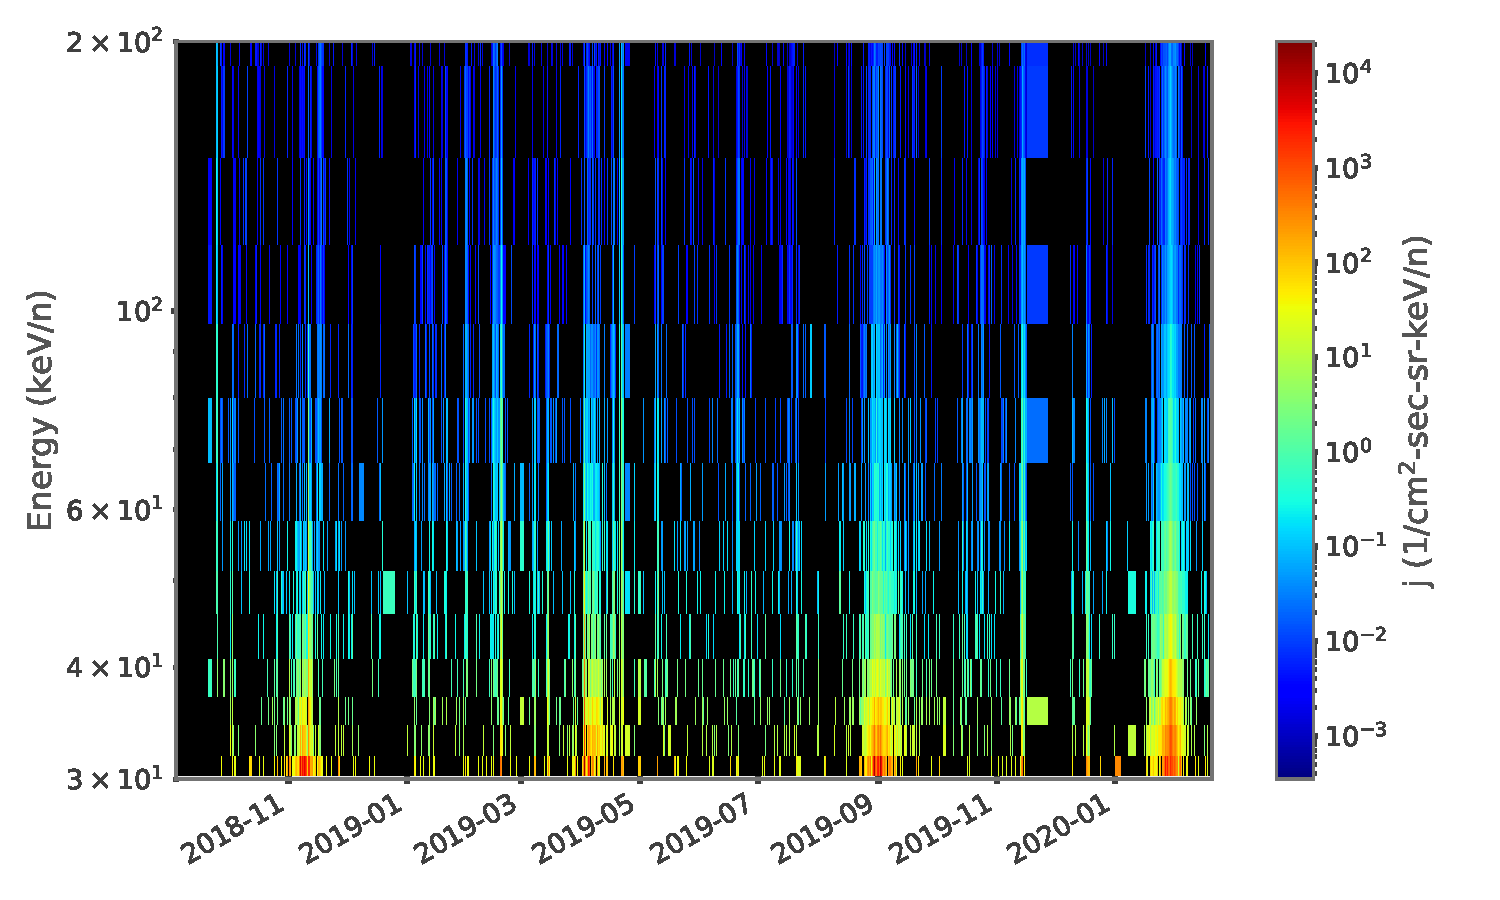
\includegraphics[width=0.9\linewidth]{figures/flux_global.pdf}
\caption{Flux (j) versus energy and time for the duration of the mission at the time data analysis was started.  Individual events generally lasted for the approximate duration of a few days, making them too small to indicate on the spectrogram.  Notice that solar encounters are visible occurring approximately every 5 months starting in November 2018.}
\label{fig:flux_global}
\end{figure}

\begin{table}[htbp]
\resizebox{\textwidth}{!}{
\begin{tabular}{ r c c c c c c }
\\
Event & Start & Stop & Spec. Index & R (\si{\astronomicalunit}) & Peak Flux (\si{n \per \kilo\electronvolt.\centi\meter\squared.\second.\steradian}) & $\eta^2$ \\
\hline
\\
       0 & 2018-09-25 01:54 & 2018-09-25 22:57 & -2.06 & 0.81 &   2.92 & 0.0327 \\ \\
       1 & 2018-11-11 01:39 & 2018-11-12 01:36 & -5.99 & 0.24 &  56.29 & 0.0345 \\ \\
       2 & 2018-11-15 16:33 & 2018-11-19 23:37 & -2.08 & 0.38 &   3.07 & 0.0161 \\ \\
       3 & 2019-01-31 00:21 & 2019-02-01 17:00 & -3.70 & 0.92 &   2.73 &    n/a \\ \\
       4 & 2019-02-13 17:43 & 2019-02-18 00:03 & -3.12 & 0.85 &   2.83 &    n/a \\ \\
       5 & 2019-02-18 05:00 & 2019-02-19 20:55 & -5.06 & 0.83 &  11.68 &    n/a \\ \\
       6 & 2019-03-06 09:17 & 2019-03-08 05:04 & -5.82 & 0.67 &   4.60 & 0.0249 \\ \\
       7 & 2019-03-13 23:33 & 2019-03-15 12:34 & -6.29 & 0.56 &   6.10 & 0.1070 \\ \\
       8 & 2019-04-02 05:44 & 2019-04-03 00:36 & -8.34 & 0.18 & 159.11 & 0.0130 \\ \\
       9 & 2019-04-04 02:36 & 2019-04-04 20:01 & -5.46 & 0.17 &  30.60 & 0.0042 \\ \\
      10 & 2019-04-17 15:36 & 2019-04-18 06:51 & -5.21 & 0.41 &   7.18 &    n/a \\ \\
      11 & 2019-04-20 10:58 & 2019-04-23 19:32 & -3.21 & 0.49 &   5.33 & 0.0112 \\ \\
      12 & 2019-06-19 15:10 & 2019-06-21 22:20 & -3.03 & 0.94 &   1.76 &    n/a \\ \\
      13 & 2019-10-22 11:09 & 2019-10-26 08:04 & -2.62 & 0.88 &   1.67 &    n/a \\ \\
      14 & 2019-11-13 08:30 & 2019-11-16 22:08 & -4.88 & 0.94 &   6.23 &    n/a \\ \\
\hline
\\
\end{tabular}}

\caption{Parameters of the fifteen events identified.  Events for which magnetic field data was unavailable show n/a for $\eta^2$.}
\label{tab:params}
\end{table}

\citet{Fisk2006} suggest a model of compressional acceleration in solar wind turbulence that predicts a functional dependence of flux on energy in the suprathermal tail as
\begin{equation}
j = j_0 T^{-3 \over 2}.
\label{eqn:flux}
\end{equation}
I attempt to recover this model from fits to the spectra of each event.

The first approach to find evidence of the model in Equation \ref{eqn:flux} fitting the spectra of the events was to simply apply a fit to the data between 40 and \SI{160}{\kilo\electronvolt} of an event-duration- and directionally-averaged spectrum of each event.  This energy region was determined by visual inspection of the events to to fit the region most like a power-law inside the suprathermal region described by \citet{Fisk2008}. This yielded fits like those shown in Figure \ref{fig:naive_fits}.  The exponents of these fits did not match well to the expected $-{3 \over 2}$.

\begin{figure}[htbp]
\centering
\begin{subfigure}{.45\textwidth}
\centering
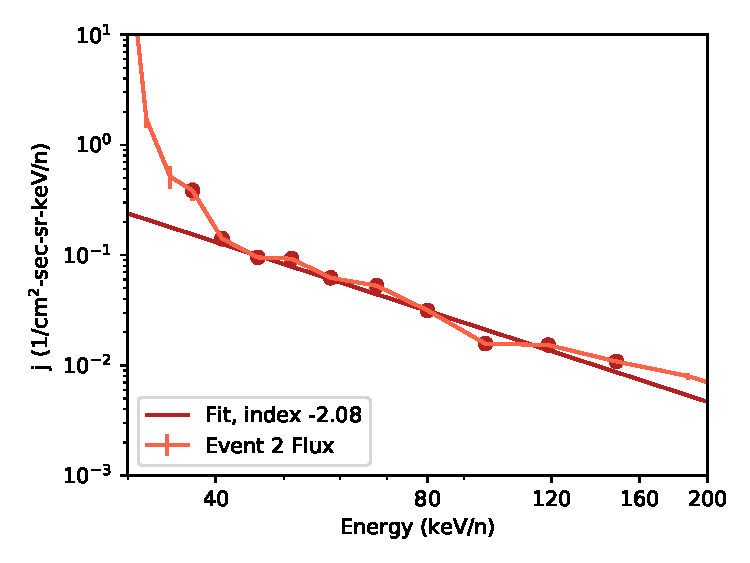
\includegraphics[width=1.\linewidth]{figures/spectrum_02.pdf}
\caption{Event 2}
\end{subfigure}
\begin{subfigure}{.45\textwidth}
\centering
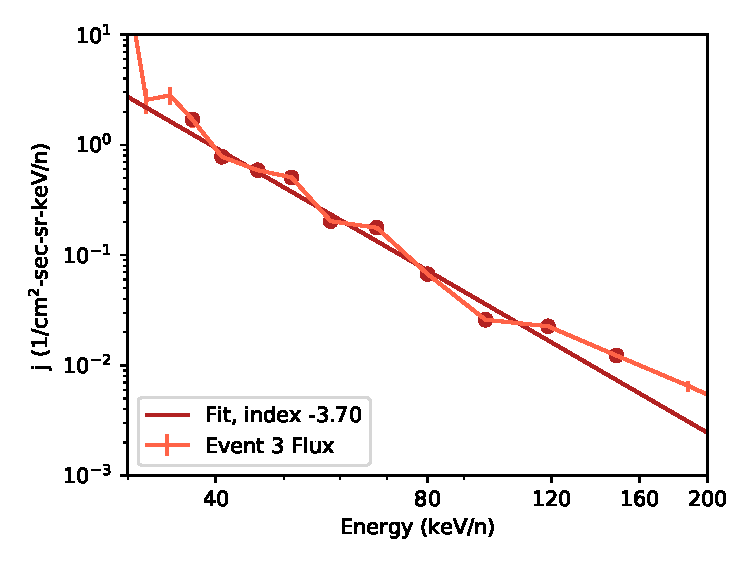
\includegraphics[width=1.\linewidth]{figures/spectrum_03.pdf}
\caption{Event 3}
\end{subfigure}
\caption{Fits of the spectra from Events 2 and  3.  Red points on the spectrum of either plot indicate points used for the fit.}
\label{fig:naive_fits}
\end{figure}

Failing to see evidence of the $-{3 \over 2}$ index of the power law, I reconsidered the importance of event type on this predicted observation.  \citet{Fisk2006} point out that the common spectrum appears in populations of charged particles subject to non-shock (ie. quiet time) acceleration, such as in gradual SEP events like those associated with coronal mass ejections.  I analyzed a combination of properties of the magnetic field to distinguish gradual SEP events from others.  

I looked at the strength of the three components of the magnetic field relative to eachother over the duration of each event to classify impulsive versus gradual SEP events.  Because the common index is associated only with gradual quiet-time SEP events, it could be necessary to eliminate events that do not fit that criterion from those being considered.  When analyzing the magnetic field a shock appears as a rapid change in the strength and direction of the magnetic field.  Qualitatively representative samples can be seen in Figure \ref{fig:b_rtn}.  Excluding events which were found to have shock-like features in the magnetic field did not yield improved statistics of the remaining spectra and associated fits.

\begin{figure}[htbp]
\centering
\begin{subfigure}{1.\linewidth}
\centering
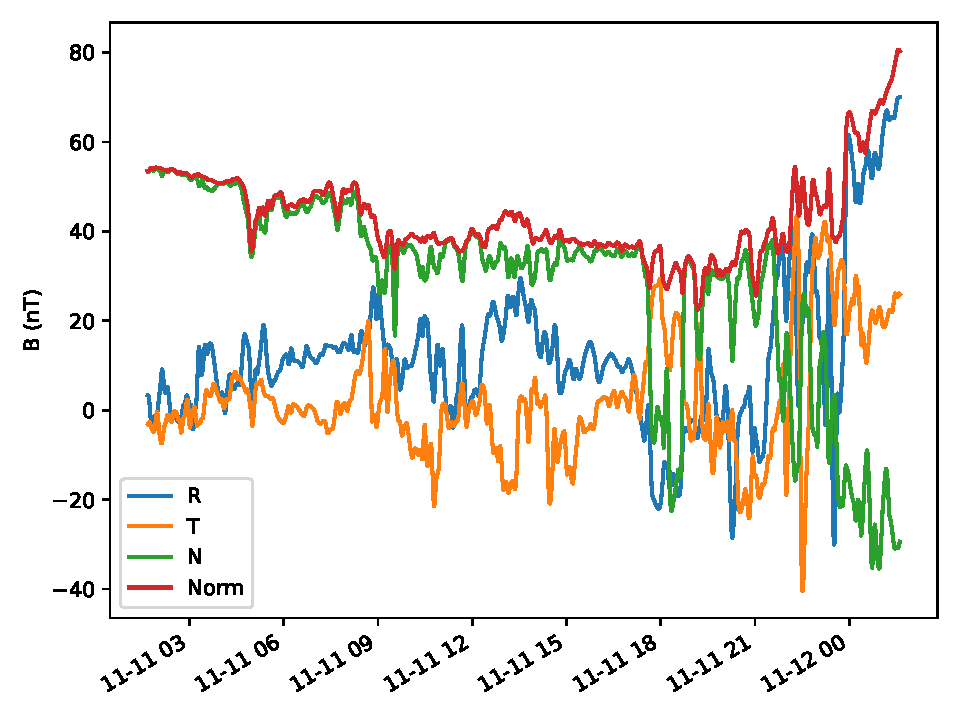
\includegraphics[width=0.75\linewidth]{figures/B_RTN_01.pdf}
\caption{Event 1. Example of a the spacecraft crossing a shock boundary.  Notice at first the strongest direction of the magnetic field is the normal.  This evolves to be the radial component by the end of the event.}
\label{fig:b_rtn_01}
\end{subfigure}
\begin{subfigure}{1.\linewidth}
\centering
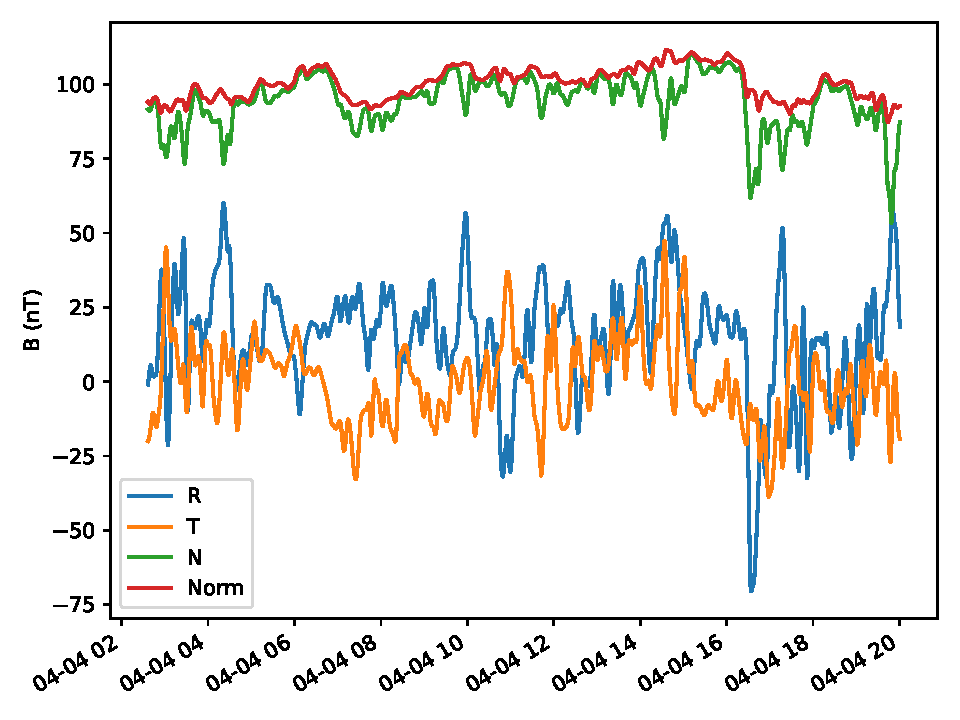
\includegraphics[width=0.75\linewidth]{figures/B_RTN_09.pdf}
\caption{Event 9.  Example of the spacecraft passing through shock-free space.}
\label{fig:b_rtn_09}
\end{subfigure}
\caption{Plots of the three components of B and its magnitude.}
\label{fig:b_rtn}
\end{figure}

I also considered magnetic variance acting as a proxy for magnetic turbulence to indicate accelerating processes in the region of the spacecraft.  \citet{Schwadron1996} suggest the statistical quantity $\eta^2$ to act as a proxy of magnetic turbulence.  Magnetic turbulence indicates the relative strength of acceleration associated with magnetic turbulence~\citep{Fisk2006}.  Plots of $\eta^2$ is shown in Figure \ref{fig:etasq}.  An association between magnetic variance and spectrum harness was not found.  However, a pattern showing events at smaller radii to have less magnetic turbulence is observed.

\begin{figure}[htbp]
\centering
\begin{subfigure}{1.\linewidth}
\centering
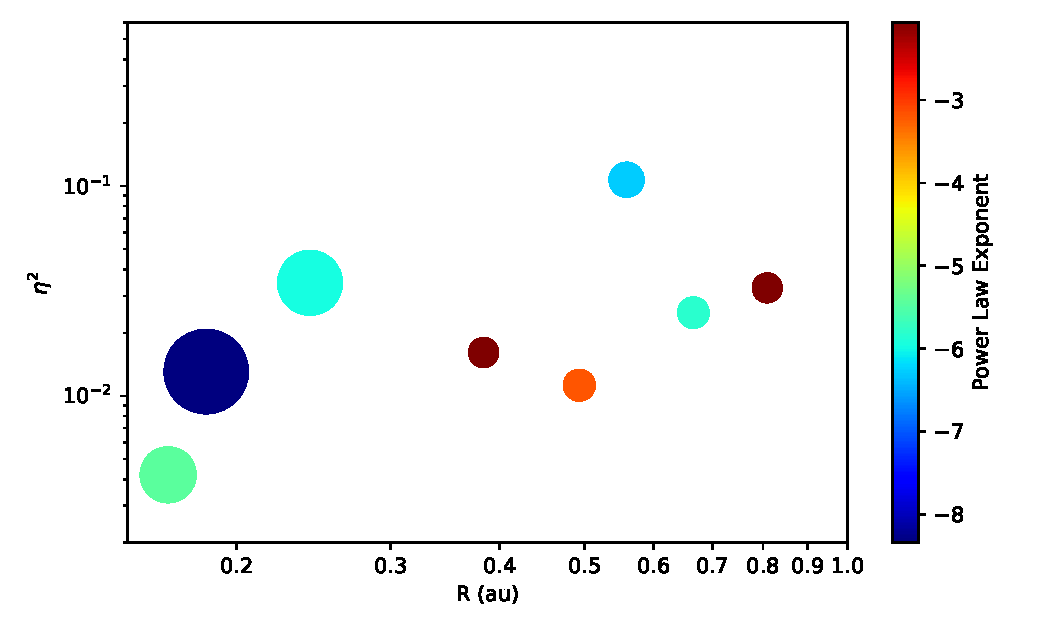
\includegraphics[width=0.9\linewidth]{figures/etasq_vs_R_events.pdf}
\caption{Variance of magnetic field versus radial distance for each event compared with its peak flux and its spectral index.  Size indicates peak flux, color indicates spectrum hardness. \citet{Schwadron1996} propose magnetic variance $\eta^2$ to be a proxy for plasma turbulence.  It appears that a trend exists such that events closer to the sun have less variance in the magnetic field.}
\label{fig:etasq_events}
\end{subfigure}
\begin{subfigure}{1.\linewidth}
\centering
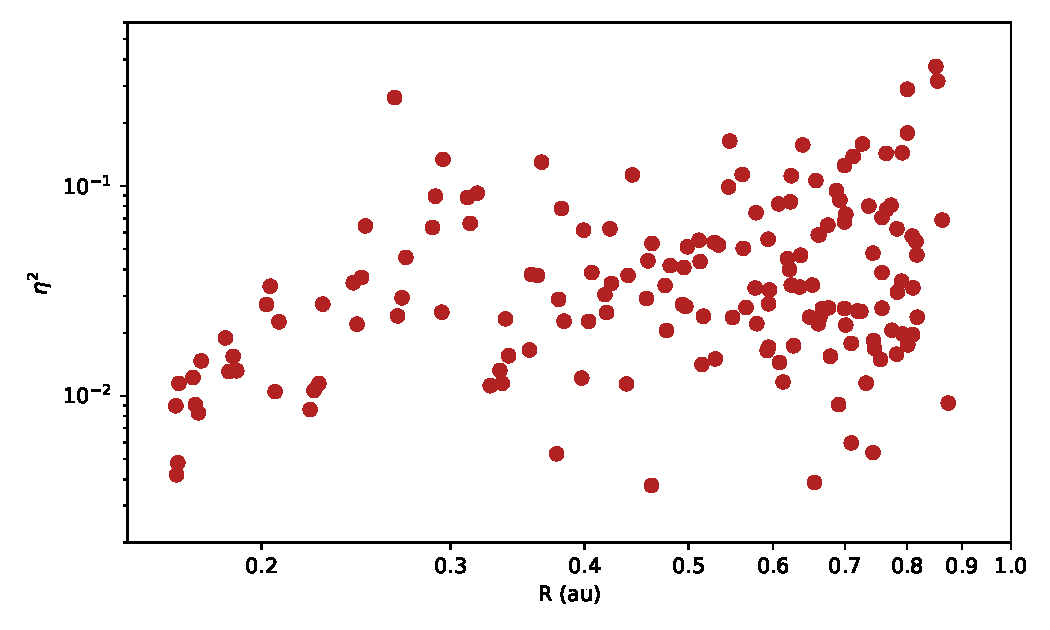
\includegraphics[width=0.9\linewidth]{figures/etasq_vs_R.pdf}
\caption{Variance of magnetic field versus radial distance for each day included in the analysis, (ie. mid September 2018 to January 2020).  The apparent upper limit of magnetic turbulence as a function of radius seen in Figure \ref{fig:etasq_events} is even more apparent here.}
\label{fig:etasq_daily}
\end{subfigure}
\caption{$\eta^2$ versus radial distance.}
\label{fig:etasq}
\end{figure}



\section{Discussion \& Conclusion}
\label{sec:conclusion}
I analyze proton flux data from Parker Solar Probe's first year and a half to find evidence for the common power law tail described in \citet{Fisk2006}.  I do not find evidence to suggest a common spectrum among these data.

I consider a naive approach without disregarding any event that may include processes originally excluded in \citet{Fisk2006}.  Failing to find the common power law tail here, I then attempt to exclude events based on changes to the magnetic field.  Manually inspecting field data for shocks and excluding associated events does not improve the net statistics of the fits to the event spectra; subsequently analyzing magnetic variance (as a proxy for magnetic turbulence \citep{Schwadron1996}) does not show any patterns in the spectral index, (see Figure \ref{fig:etasq}).



\section{Future Work}
\label{sec:future}
Some extensions to this study could include the following:

\begin{itemize}
\item Analysis on a moving average of each event may show different results or evidence of the common spectrum.  Upon writing, it became apparent that the spectra of many events harden as time goes on, (ie. the exponent of spectrum, if the range of the spectrum is taken to move in time, increases from more negative to less negative).
\item Compare events with other authors and observatories and exclude events on this basis.
\end{itemize}



\section{Acknowledgments}
The author wishes to sincerely thank Dr. Jonathan Niehof and Professor Nathan Schwadron for sharing their expertise and guidance throughout the research process, without which this work could not have been accomplished. In addition, the author would like to thank Dr. Dana Filoti and Professor James Ryan for their feedback during the University of New Hampshire Undergraduate Research Conference in Physics.

\bigskip

\noindent This work was supported by NASA Prime Contract No. 136435.



\bibliographystyle{thesis}
%\bibliographystyle{abbrv}
%\bibliographystyle{plainnat}
\bibliography{thesis}

\end{document}
